\subsubsection{Testprotokoll: Latenzmessung}
\label{test-latenzmessung}

Messung der Latenz vom Zeitpunkt des Triggerinputs bis zur Audioausgabe über den Audio-Codec.

Durchführung mit dem STM32-Audioprojekt aus dem Repository (\href{run:../../f401_sd_card_audio_codec_test/}{\texttt{/f401\_sd\_card\_audio\_codec\_test/}}).
Der Audio-Codec, sowie der SD-Kartenleser müssen wie im Schaltplan(TODO: REFERENZ auf Schaltplan) verbunden werden.

\paragraph{Schritte:}
\begin{enumerate}
	\item Anschluss zweier Oszilloskop-Sonden: an Trigger-Input/Play-Button-Pin und Audio-Ausgang.
	\item Laden einer Test PCM .wav-Datei mit einer Samplerate von \SI{44.1}{\kilo\hertz}, 16 Bit und Stereo/2 Kanälen auf die SD-Karte.
	\item Umschalten des Oszilloskops in den Single-Shot-Modus und Konfiguration zur Auslösung durch den Audio-Kanal.
	\item Abspielen der Testdatei durch Auslösen des Play-Buttons.
	\item Positionierung zweier Mess-Cursor: einer auf die erste Flanke des Trigger-Input-Signals und der andere auf den Beginn des Audio-Ausgangssignals.
\end{enumerate}
\paragraph{Erwartete Werte}
	Die erwartete Latenz errechnet sich wie folgt:
	
	\textit{Gegeben:}
	\begin{align*}
		\text{Samplerate} &= \SI{44.1}{\kilo\hertz} = 44{,}100 \, \text{Samples pro Sekunde} \\
		\text{Puffergröße} &= 256 \, \text{Samples}
	\end{align*}
	
	\textit{Berechnung der Latenz:}
	
	\[
	\text{Zeit pro Sample} = \frac{1 \, \text{Sekunde}}{44{,}100 \, \text{Samples}} \approx \SI{22.68}{\micro\second}
	\]
	
	\[
	\text{Zeit für einen Puffer} = 256 \, \text{Samples} \times \SI{22.68}{\micro\second} \approx \SI{5.8}{\milli\second}
	\]
	
	Die Latenz für das System mit den angegebenen Parametern beträgt also im Idealfall \( \SI{5.8}{\milli\second} \).
	
\paragraph{Testergebnisse}

\begin{itemize}
	\item Gemessene Latenz von \SI{6.4}{\milli\second} (\textbf{BX-AX} in Abbildung  \ref{fig:audio-latency-test}).
	\item Die Abweichung von der erwarteten Latenz ist wahrscheinlich auf die Verarbeitungszeiten des Audio-Codecs zurückzuführen.
	\item Sehr praktikabler Latenzwert für Audioinstrument.
\end{itemize}

\begin{figure}[H]
	\centering
	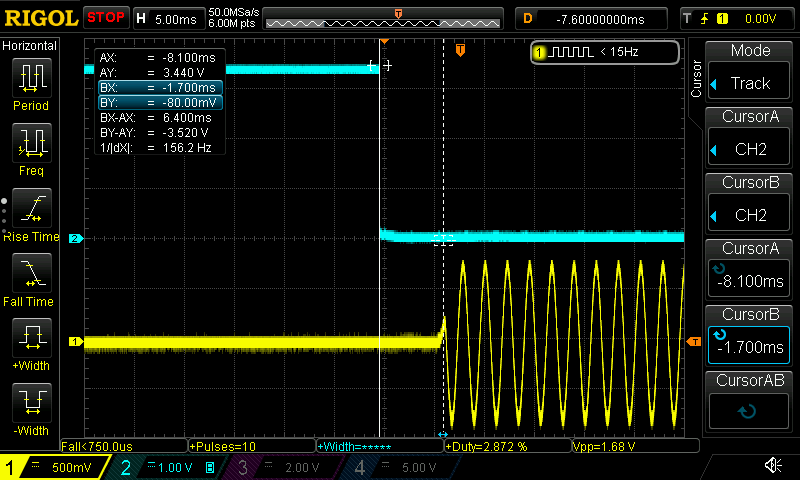
\includegraphics[width=0.6\textwidth]{images/10_test_validierung/audio/audio-latency-test.png}
	\caption{Oszilloskopansicht der Latenzmessung von Trigger (Blau) bis Audioausgang (Gelb)}
	\label{fig:audio-latency-test}
\end{figure}